\documentclass[12pt]{article}
\usepackage{sbc-template}
\usepackage{graphicx}
\usepackage[obeyspaces,spaces]{url}
\usepackage[brazil]{babel}
\usepackage[utf8]{inputenc}
\usepackage{paralist}
\usepackage{listingsutf8}
\usepackage{subfigure}

\setlength{\abovecaptionskip}{6pt}
\setlength{\belowcaptionskip}{6pt}

\sloppy

\title{Pelo fim da violência contra a mulher\\Uma estratégia com uso de Redes Sociais}

\author{Alexandre D. Rogoski, Guilherme Enoc,\\Guilherme H. P. Gonçalves, Maycon Sambinelli, Otávio Siste}

\address{Departamento de Informática\\
  Universidade Estadual de Maringá (UEM) -- Maringá, PR -- Brasil
  \email{alexandre@exatati.com.br,\\\{guiegas,ggpolo,msambinelli,otaviosiste\}@gmail.com}
}

\begin{document}

\maketitle

\begin{abstract}
% The best thing since sliced bread <:)
\end{abstract}

\begin{resumo}
\end{resumo}

% Início conteúdo
\section{Introdução}


\section{Violência contra a mulher} % [GP]
Seguindo o dossiê de \cite{dossie}, encontra-se a seguinte definição de como
a violência tem sido entendida:
``uma ação praticada que envolva a lesão, seja ela física,
psicológica, simbólica ou sexual, à integridade da vítima''. Infelizmente
a verificação dessa definição ocorre rotineiramente, sendo distribuída
continuamente pelos meios de comunicação. Pelo menos 15 conceituações sobre
formas de aplicar a violência podem ser encontradas por meio deste mesmo
dossiê. Destinando-se especificamente a violência contra a mulher,
o dossiê define todos estes conceitos e entre eles estão: violência
sexual, violência psicológica, violência doméstica, violência física,
discriminação contra a mulher, violência de gênero, violência institucional,
entre outros. O penúltimo dos conceitos mencionados refere-se a ``violência
aplicada sem distinção de raça, classe social, religião, idade ou qualquer
outra condição, produto de um sistema social que subordina o sexo
feminino'' \cite{dossie}. A última forma mencionada trata da violência
oriunda dos órgãos e agentes públicos. Fica claro que a violência tem
ocorrido com tanta frequência e dos mais diversos modos que foi
necessário a criação de classificações específicas. Ao longo dessa
seção será discutido essa forma de violência com enfoque no Brasil.

Desde 1994, por meio da Convenção Interamericana para prevenir, punir e
erradicar a violência
contra a mulher \cite{interamericana}, o Brasil e os demais 34 países membros
da OEA (Organização dos Estados Americanos) têm definido os deveres do
país, mecanismos de proteção, direitos protegidos e definições a cerca da
violência contra a mulher. Ficou definido que a violência contra a mulher
é ``qualquer ação ou conduta, baseada no gênero, que cause morte, dano ou
sofrimento físico, sexual ou psicológico à mulher, tanto no âmbito
público como no privado''. E que toda mulher tem direito a uma vida livre
de violência, tanto no âmbito público como no privado. Ainda foi estabelecido
que em todo o território nacional é condenado todas as formas de
violência contra
a mulher e concorda-se em adotar, por todos os meios apropriados e sem demora,
políticas voltadas a prevenção, punição e erradicação desta forma de violência.
Entre os mecanismos de proteção foi dito que qualquer pessoa ou grupo de
pessoas, ou entidade não-governamental legalmente reconhecida, pode apresentar
à Comissão Interamericana de Direitos Humanos petições que contenham denúncias
ou queixas de violação do Artigo 7 do documento em discussão. Entretanto, não
está claro quais ações estão previstas para os denunciados.

De modo geral pode-se dizer que a sociedade brasileira atualmente condena a
violência física contra a mulher, devido a efeito de resultados partindo
da Convenção mencionada acima ou não. A pesquisa realizada
por \cite{ibope1} exibe a estatística de que ``91\% dos brasileiros
consideram muito grave o fato de mulheres serem agredidas por
companheiros e maridos''. Ainda, 90\% dos entrevistados ``acham que
o agressor deveria sofrer um processo e ser encaminhado para uma
reeducação''. Por um lado o povo parece estar consciente dessa forma
de violência e de que punições devem ser aplicadas. Por outro lado,
o estudo de \cite{avon1} indica que a cada 15 segundos uma mulher é agredida e,
assim, revela algum problema mais grave com a sociedade. Um dos pontos
favoráveis a tanta violência pode estar relacionado ao fato de que mais
da metade, 56\% de acordo com \cite{avon1}, de uma parcela representativa
da população tem a opinião de que a mulher não pode confiar na proteção
jurídica e policial existente no Brasil.
Ou seja, a impunidade (ou ao menos a sensação da mesma) pode estar
favorecendo mais essa prática.
Entretanto, há outros problemas mencionados. Para outros 38\%, o álcool é o
fator que leva a violência doméstica. Além disso, outros 36\% acreditam que a
cultura do homem brasileiro é naturalmente violenta. Sendo um fator cultural
este último, a pesquisa tentou buscar opiniões a cerca do que poderia
ser feito para reduzir esses números. Cerca de metade
(48\% desta mesma pesquisa) dos entrevistados acreditam que o mais
importante para o ajuste cultural esteja relacionado aos pais darem
o exemplo de relacionamento respeitoso e igualitário.

Já a agressão unicamente psicológica (aquela que não faz uso da
violência física), baseando-se na pesquisa acerca de material
relacionado, parece ser bem menos comentada além de ser mais difícil
de comprovar. Ainda assim, o artigo de \cite{penha1} diz que essa é a
forma mais comum de violência e mais danosa que a própria violência
física. Uma forma de violência psicológica atualmente bastante
conhecida é o \textit{bullying}, que pode ocorrer em qualquer lugar
onde hajam pessoas que interagem. Porém, diferentemente da violência
física, aqui não há uma dominância
clara de quem é mais agredido ou de quem agride mais.

Independente da violência sofrida,
pode-se pensar que a vítima imediatamente rompa
relações existentes com o agressor. Entretanto, esse não é o caso. Na
pesquisa apresentada em \cite{ibope1}, as 4 opiniões que lideraram o motivo
por não haver esse rompimento foram:
falta de condições econômicas para viver sem o companheiro (24\%),
preocupação com a criação dos filhos (23\%), medo de morte
caso rompa a relação (17\%), falta de auto-estima (12\%). Com outros
dados ali apresentados, verifica-se que entre todos os entrevistados, a maior
porcentagem daqueles que opinaram por ``medo de morte'' representam os
indivíduos de menor poder aquisitivo, baixa escolaridade e de idade entre
16 e 24 anos. Ou seja, muitas mulheres vivem em real situação de risco.
O reflexo direto dessa situação é de que, de acordo com \cite{avon1},
a violência doméstica tem sido considerado o problema mais preocupante
para as mulheres brasileiras. Em 2006, 50\% das mulheres consideravam este
como o tópico mais problemático e em 2009 passou para 56\%. Até mesmo
assuntos como AIDS e câncer de mama e útero ficaram atrás na pesquisa.

As consequências desta violência são as mais diversas. O texto em
\cite{outlook1} apresenta um ciclo da violência contra a mulher ao
longo de sua vida e
seus efeitos sobre a saúde, que pode ser visto na figura \ref{fig:ciclov}.
\begin{figure}[ht]
  \centering
  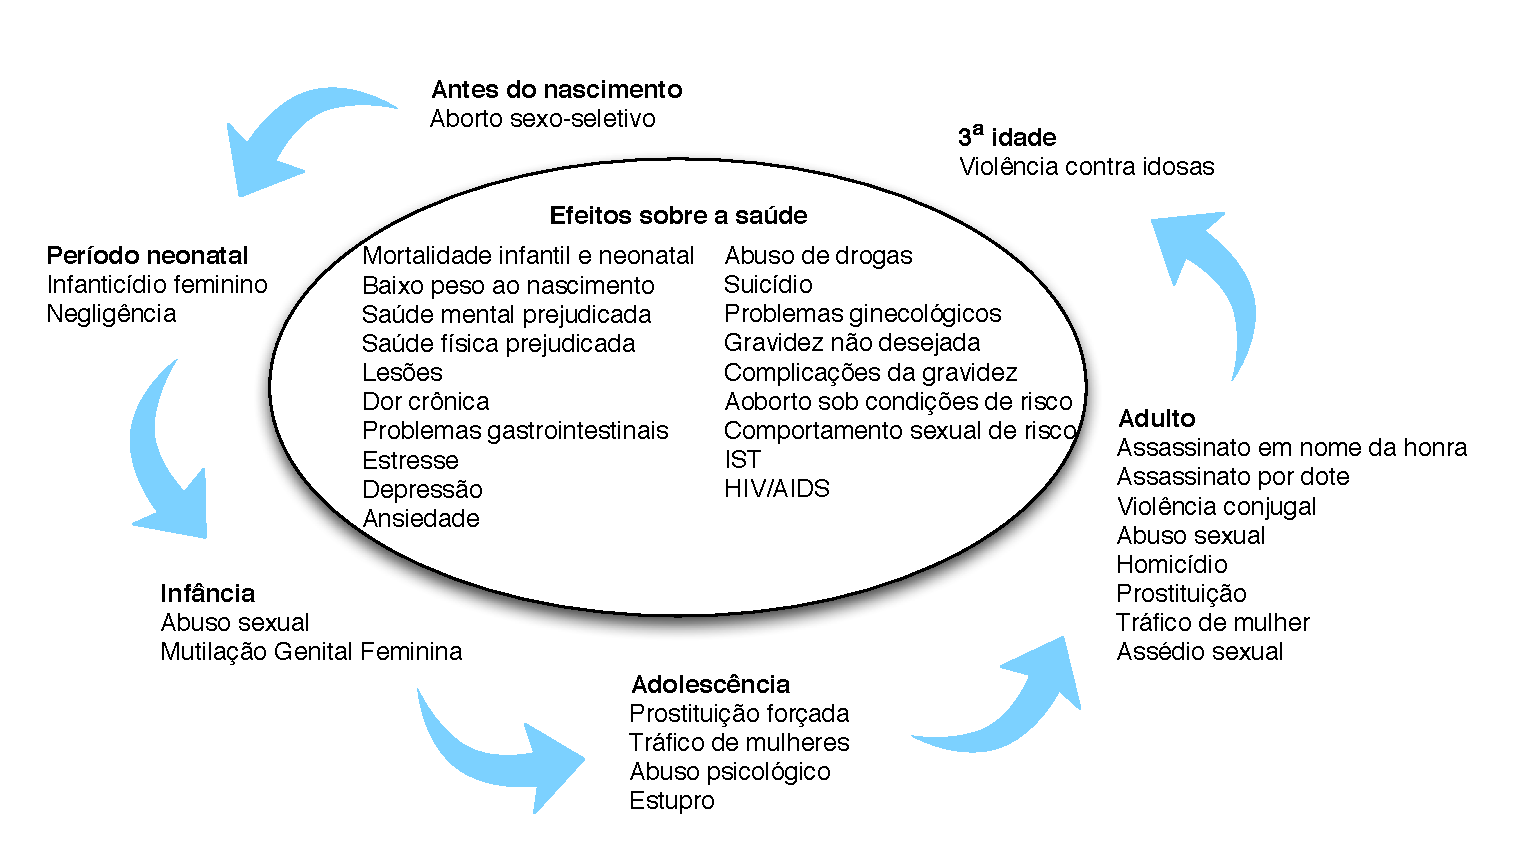
\includegraphics[width=\linewidth]{cicloviolencia}
  \caption{A violência contra a mulher em seu ciclo de vida e os
    efeitos sobre a saúde \label{fig:ciclov}}
\end{figure}
Existe, assim, a possibilidade da violência iniciar-se antes mesmo do
nascimento e continuar durante toda a vida. O impacto da violência
pode ser tanto imediato quanto de longo prazo, sendo que as
sobreviventes muitas vezes desenvolvem a prática de uso de álcool e
drogas \cite{outlook1}. Também há ocorrência de dores crônicas,
problemas e sintomas neurológicos (desmaios e convulsões, por
exemplo), distúrbios gastrointestinais e problemas cardíacos. Além
disso, as mulheres agredidas frequentemente vivem com medo,
desenvolvem depressão, ansiedade e síndrome do estresse
pós-traumático. Um estudo da OMS (Organização Mundial de Saúde) feito
no Brasil (além de outros países) mostrou que mulheres que haviam
sofrido abuso físico ou sexual pelos seus parceiros pensavam duas
vezes mais em suicídio quando comparadas àquelas que não haviam sofrido
nenhuma forma de abuso. O trabalho apresentado em \cite{hopkins1} diz
ainda que as sobreviventes a esses tipos de atos têm maior
probabilidade de adotarem comportamentos sexuais de alto risco
(prostituição, múltiplos parceiros, entre outros) e consequentemente
gravidez indesejada e/ou HIV (\textit{Human Imunodeficiency Virus}) e
IST (Infecções Sexualmente Transmissíveis).

Um ponto positivo no Brasil é a verificação de que não mais aguarda-se
pelo poder público
quando o assunto tratado é a violência contra a mulher,
felizmente. Diversas organizações têm surgido e atuado com o objetivo
de erradicar este problema social. De acordo com o trabalho feito em
\cite{avon1}, há 6 organizações mais atuantes no país: Instituto Patrícia
Galvão (\url{http://www.patriciagalvao.org.br}), Comitê Latino Americano e do Caribe para a Defesa dos Direitos
da Mulher (Cladem -- \url{http://www.cladem.org}), Centro Feminista de
Estudos e Assessoria (CFEMEA -- \url{http://www.cfemea.org.br}),
CEPIA (Cidadania, Estudo, Pesquisa, Informação, Ação --
\url{http://www.cepia.org.br}), Fundação Perseu
Abramo (\url{http://www.fpabramo.org.br}), Themis -- Assessoria
Jurídica e Estudos de Gênero. A última
dessas é uma ONG fundada em 1993 que ``busca no Direito e na
Capacitação Legal, a
efetivação dos direitos humanos das mulheres através do acesso a
justiça, contribuindo assim, com a superação das desigualdades
sociais'' (\url{http://www.themis.org.br/}). É possível que esse seja
um modo de reverter a situação em relação a sensação de impunidade
existente. As demais organizações, de forma geral, tem como intuito
promover o acesso a informações relacionadas a esse tópico e também
fortalecer políticas de combate a agressão e assistência a vítima.

\subsection{Casos de violência contra a mulher}


\section{Lei Maria da Penha}


\section{Combate a violência contra a mulher}


\section{Uso de redes sociais para ajudar a erradicar a violência
  contra a mulher}

\subsection{Redes sociais}
% + O que são redes sociais % [OS]
% + Importância das redes sociais: % [AL]
% + Algum protesto relevante que ocorreu em redes sociais e que teve
%   um significado forte % [MS]

% + Quantidade de pessoas que estão conectadas em redes sociais % [GP]
% - Redes sociais e seus percentuais de usuários (quantos % porcento
%   tem cada rede social ) % [GP]
%    + Por faixa etária
%    + Classe social
Uma pesquisa realizada pela Nielsen (\url{http://www.nielsen.com/}) em
2009 \cite{nielsen1} mostrou que dois terços da população
mundial\footnote{Estados Unidos, Brasil, Reino Unido, França,
  Alemanha, Itália, Espanha, Suíça e Austrália -- países onde a Nielsen
  faz uso de seu serviço NetView}, que
dispõe de acesso a Internet, visita rede social ou
\textit{blogs} e gasta quase 10\% de todo o tempo consumido na
Internet. Isso significa que esses sites já superam o tempo gasto com
email, ficando atrás somente dos setores de busca (Google, por ex.),
portais (UOL, Terra, etc) e
aplicativos de uso geral (editores de texto, por ex.). De acordo com
as métricas da Nielsen, a rede social \texttt{Facebook} é a líder
mundial, sendo acessada por 3 a cada 10 pessoas \textit{on-line}.
Algo ainda, talvez,
mais assustador surge se considerarmos uma pesquisa realizada pela
comScore (\url{http://www.comscore.com}) em Agosto de 2010 no Brasil
\cite{comscore1}. Nesta pesquisa foi constatado a presença de pouco
mais de 37 milhões e 500 mil usuários de Internet no Brasil com 15
anos ou mais, onde mais de 36 milhões (ou seja, mais de 96\% do total)
visitaram redes sociais. O brasileiro também surpreende no tempo gasto
com redes sociais, chegando a 20\% do tempo total gasto
\textit{on-line}. Esta pesquida da comScore não considerou tráfego
originado de computadores públicos (como \textit{cyber} cafés ou celulares).

Focando-se no Brasil, discutimos informações a respeito de redes
sociais. De acordo com os dados da pesquisa \cite{comscore1}, as três
redes sociais mais acessadas no Brasil são, em ordem de maior acesso:
\texttt{Orkut}, \texttt{Facebook}, \texttt{Twitter}. Dados adiante serão
dedicados exclusivamente a essas três redes. A figura \ref{fig:redes1}
apresenta a quantidade de usuários distintos que
acessaram cada site e em \ref{fig:redes2} é apresentado o tempo médio
que cada usuário permaneceu nesses sites durante o mês todo.

\begin{figure}[ht]
  \centering
  \subfigure[Visitas únicas (milhões)\label{fig:redes1}]{\includegraphics[width=0.42\linewidth]{redessociais_0_gray}}
  \qquad
  \subfigure[Tempo médio de permanência (minutos)\label{fig:redes2}]{\includegraphics[width=0.425\linewidth]{redessociais_1_gray}}
  \caption{Redes sociais mais visitadas em Agosto de 2010 -- Brasil \label{fig:dados1}}
\end{figure}

O \texttt{Orkut}
foi um dos destinos de cerca de 78\% (mais de 29 milhões) do total de
pessoas \textit{on-line} no país durante um mês. Na média, os usuários
do \texttt{Orkut} gastaram mais de 4 horas e meia (275,8 minutos) ao
longo do mês nesta rede social. As outras redes ficaram bastante
distantes dos números desta, mas o \texttt{Facebook} cresceu 479\% em
relação ao ano passado de acordo com a pesquisa. Além disso, o
\texttt{Twitter} atingiu cerca de 23\% da população com acesso a
Internet no Brasil; resultado esse que coloca o Brasil como o país que
mais utiliza o \texttt{Twitter} em porcentagem de usuários.

Continuando com esta pesquisa da comScore \cite{comscore1},
apresentamos a figura \ref{fig:dados2}. Em \ref{fig:redes3} é exibido
o número de páginas do site que cada usuário visitou, em média,
durante um mês. Na \ref{fig:redes4} é
apresentado o número de vezes em média que cada usuário visitou o
respectivo site. Nota-se que apesar do \texttt{Orkut} ter uma
quantidade superior de páginas visitadas em média, ao calcular a razão
$\frac{\mathrm{tempo\,\,perman\hat{e}ncia}}{\mathrm{p\acute{a}ginas\,\,visitadas}}$
verifica-se que os usuários do \texttt{Twitter} são os que apresentam
a maior permanência, em média, por página: cerca de 43
segundos. Talvez esta razão esteja indicando que há uma busca
excessiva por conteúdo e que, talvez, poucas páginas acessadas são
realmente lidas. % Se a gente quer propor algo com redes sociais, tem
                 % que ser algo bem rápido de visualizar e chamar a
                 % atenção já.

\begin{figure}[ht]
  \centering
  \subfigure[Média de páginas/usuário\label{fig:redes3}]{\includegraphics[width=0.42\linewidth]{redessociais_2_gray}}
  \qquad
  \subfigure[Média de visitas/usuário\label{fig:redes4}]{\includegraphics[width=0.42\linewidth]{redessociais_3_gray}}
  \caption{Média de páginas e visitas por visitante nas redes sociais
    no Brasil \label{fig:dados2}}
\end{figure}

Em relação a consumo de conteúdo, a pesquisa em \cite{comscore1}
apresenta dados por idade, gênero e região. De modo geral, as mulheres
consomem mais conteúdo em redes sociais. Os mais jovens, aqueles entre
15 e 24 anos, consomem mais conteúdo do que um visitante mediano nas
redes \texttt{Orkut} e \texttt{Twitter}. A rede \texttt{Facebook} foi
aquela onde usuários de idade a partir de 25 anos mostrarem-se mais
ativos. Esses e outros dados podem ser vistos na figura
\ref{fig:redes5}. % Não falei sobre consumo por região na verdade.

\begin{figure}[ht]
  \centering
  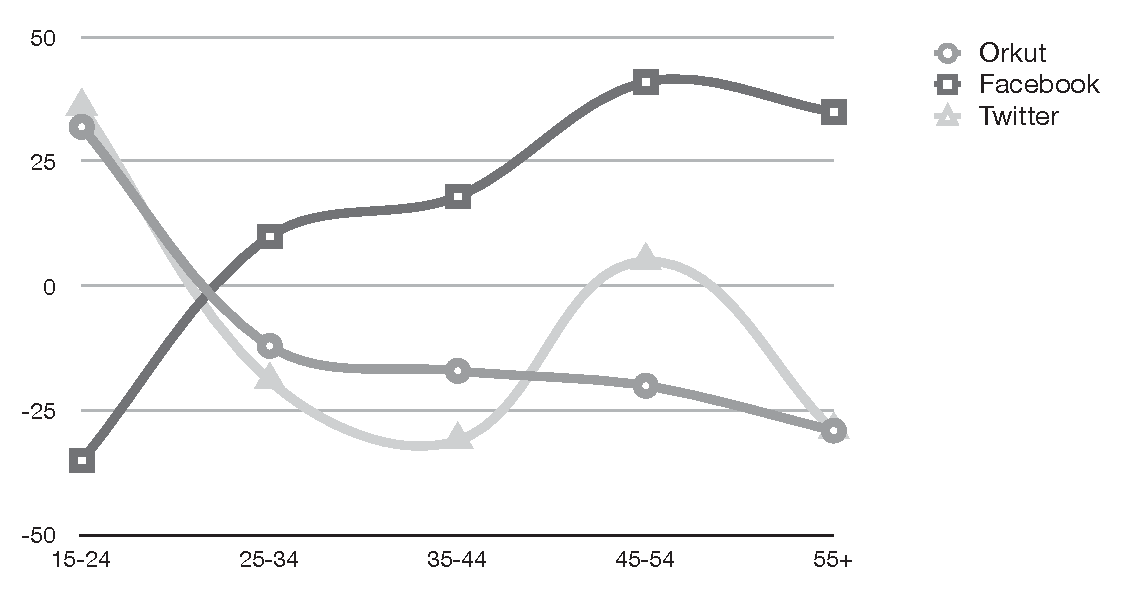
\includegraphics[width=0.86\linewidth]{redessociais_4_gray}
  \caption{Consumo de conteúdo por idade sobre consumidor mediano (\%) \label{fig:redes5}}
\end{figure}

\begin{figure}[ht]
  \centering
  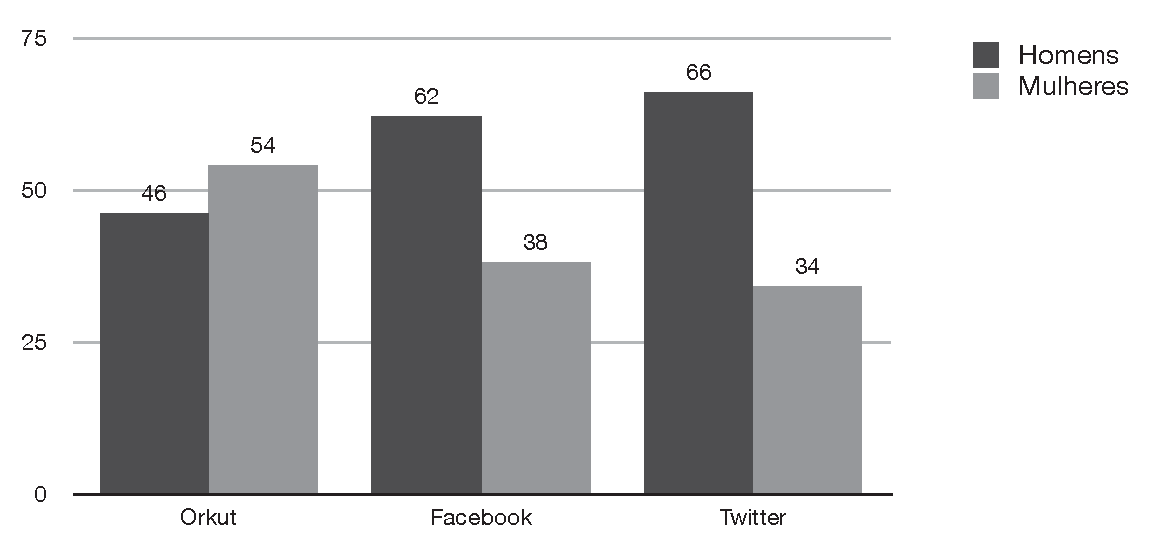
\includegraphics[width=0.84\linewidth]{redessociais_genero_gray}
  \caption{Percentual de acessos por gênero \label{fig:redes-genero}}
\end{figure}

Por meio do site \textit{DoubleClick Ad Planner} -- Google
\cite{doubleclick} buscou-se dados em relação a quantidade de acessos
por sexo. A figura \ref{fig:redes-genero} apresenta estas
informações para setembro de 2010. Entras as 3 redes estudadas, o
\texttt{Orkut} foi a única
que mostrou maior quantidade de acessos por parte das
mulheres.

\section{Conclusão}




% Referências
\bibliographystyle{sbc}
\bibliography{biblio}
\end{document}
